%% LyX 2.3.7 created this file.  For more info, see http://www.lyx.org/.
%% Do not edit unless you really know what you are doing.
\documentclass[english,xcolor=svgnames, handout]{beamer}
\usepackage{amstext}
\usepackage{fontspec}
\setcounter{secnumdepth}{3}
\setcounter{tocdepth}{3}
\usepackage{calc}
\usepackage{graphicx}
\usepackage{microtype}
\ifx\hypersetup\undefined
  \AtBeginDocument{%
    \hypersetup{unicode=true}
  }
\else
  \hypersetup{unicode=true}
\fi

\makeatletter

%%%%%%%%%%%%%%%%%%%%%%%%%%%%%% LyX specific LaTeX commands.
\providecommand\textquotedblplain{%
  \bgroup\addfontfeatures{RawFeature=-tlig}\char34\egroup}

%%%%%%%%%%%%%%%%%%%%%%%%%%%%%% Textclass specific LaTeX commands.
% this default might be overridden by plain title style
\newcommand\makebeamertitle{\frame{\maketitle}}%
% (ERT) argument for the TOC
\AtBeginDocument{%
  \let\origtableofcontents=\tableofcontents
  \def\tableofcontents{\@ifnextchar[{\origtableofcontents}{\gobbletableofcontents}}
  \def\gobbletableofcontents#1{\origtableofcontents}
}

%%%%%%%%%%%%%%%%%%%%%%%%%%%%%% User specified LaTeX commands.
\mode<presentation> {
  \usetheme{Luebeck}
  \usecolortheme{beaver}
  \beamertemplatenavigationsymbolsempty
}

\usepackage[many]{tcolorbox}
\usepackage{graphicx}
\usepackage{pgf}
\usepackage{colortbl}
\usepackage{emoji}
\usepackage{tabularx}
\usepackage{colortbl}
\usepackage{array}
\tcbuselibrary{skins}

\date{}

\definecolor{blue}{RGB}{38, 122, 181}
\definecolor{orange}{RGB}{255, 128, 0}
\definecolor{lorange}{RGB}{255, 178, 102}
\definecolor{llorange}{RGB}{255, 229,204 }
\definecolor{verylightgray}{RGB}{246, 246, 246}
\definecolor{cobalt}{HTML}{0047AB}
\definecolor{lightsteelblue}{HTML}{b0c4de}
\definecolor{burntoranger}{HTML}{CC5500}

\setbeamertemplate{itemize item}{\color{orange}$\blacksquare$}
\setbeamertemplate{itemize subitem}{\tiny \color{lightgray}$\blacksquare$}

\newcommand\boldblue[1]{\textcolor{cobalt}{\textbf{#1}}}
\newcommand\boldorange[1]{\textcolor{burntoranger}{\textbf{#1}}}
\def\*#1{\mathbf{#1}}

\newcolumntype{Y}{>{\raggedleft\arraybackslash}X}
\tcbset{tab2/.style={enhanced, fontupper=\small,
colback=lightgray!10!white,colframe=cobalt!50!black,colbacktitle=lightsteelblue!40!white,
coltitle=black,center title}}


\newcommand\blfootnote[1]{%
  \begingroup
  \renewcommand\thefootnote{}\footnote{#1}%
  \addtocounter{footnote}{-1}%
  \endgroup
}

\setbeamerfont{footnote}{size=\tiny}
\setbeamertemplate{footnote}{%
  \parindent 1em\noindent%
  \raggedright
  \insertfootnotetext\par%
}

\makeatother

\usepackage{polyglossia}
\setdefaultlanguage[variant=american]{english}
\begin{document}
\title[\textcolor{gray}{ST1101 \hspace{4.45cm}\insertframenumber/\inserttotalframenumber}]{\textcolor{orange}{Statistik och Dataanalys I}}
\subtitle{\textcolor{orange}{Föreläsning 11 - Osäkerhet och Sannolikhet}}
\author[\textbf{\textcolor{gray}{Statistik och Dataanalys I}}]{\textbf{Oscar Oelrich} \\
\vspace{0.2cm}
\vspace{-0.3cm}
}
\institute[Stockholms universitet]{Statistiska institutionen\\
Stockholms universitet}

\makebeamertitle

\begin{frame}{\textbf{\textcolor{orange}{Översikt}}}
\begin{itemize}
\item \textbf{\textcolor{blue}{Motivation}}\medskip{}
\item \textbf{\textcolor{blue}{Försök, Utfall och Händelser}}\medskip{}
\item \textbf{\textcolor{blue}{Sannolikheter}}\medskip{}
\item \textbf{\textcolor{blue}{Sannolikhetsberäkningar}}\medskip{}
\item \textbf{\textcolor{blue}{Kombinatorik}}
\end{itemize}
\end{frame}

\begin{frame}{\textbf{\textcolor{orange}{Sannolikheter för dataanalys}}}
\begin{itemize}
\item \textbf{\textcolor{blue}{Sannolikhetslära}} är intressant i sig:\medskip{}

\begin{itemize}
\item Sannolikheten för en kärnkraftsolycka \includegraphics[scale=0.03]{figs/flaticons/radiation}\medskip{}
\item Sannolikheten att två personer har identiska DNA. \includegraphics[scale=0.03]{figs/flaticons/dna}\medskip{}
\item Sannolikheten att träffa den rätta på dejtingapp. 
\includegraphics[scale=0.03]{figs/flaticons/romeo-and-juliet}\bigskip{}
\end{itemize}
\item Sannolikhetslära viktigt för \textbf{\textcolor{orange}{dataanalys}}:\medskip{}

\begin{itemize}
\item \textbf{\textcolor{blue}{Statistiska modeller är sannolikhetsmodeller}}.
\\
\smallskip{}
Bra modell av verkligheten: data sannolika enligt modellen.\medskip{}
\item Kan \textbf{\textcolor{blue}{kvantifiera}} \textbf{\textcolor{blue}{osäkerheten}}
i en \textbf{\textcolor{blue}{prediktion}}.\medskip{}
\item Kan \textbf{\textcolor{blue}{fatta optimala beslut i en osäker värld}}.\bigskip{}
\end{itemize}
\end{itemize}
\begin{center}
\begin{minipage}[t]{0.75\columnwidth}%
\begin{center}

\includegraphics[scale=0.03]{figs/MnistTest7} $\;$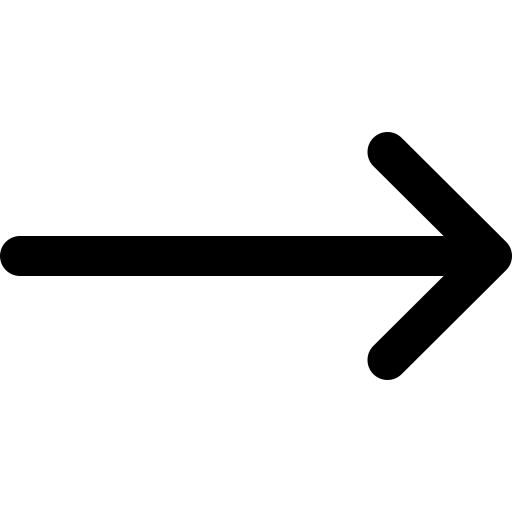
\includegraphics[scale=0.06]{figs/flaticons/right-arrow}
$\;$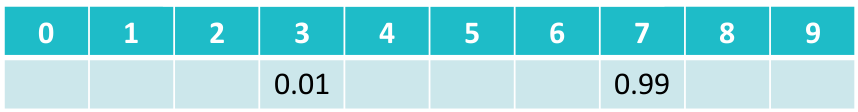
\includegraphics[scale=0.18]{figs/mnist_pred7}
\par\end{center}%
\end{minipage}%
\begin{minipage}[t]{0.05\columnwidth}%
\begin{center}
\par\end{center}%
\end{minipage}%
\begin{minipage}[t]{0.2\columnwidth}%
\begin{center}
\includegraphics[scale=0.045]{figs/flaticons/interest}
\par\end{center}%
\end{minipage}
\par\end{center}

\end{frame}

\begin{frame}{\textbf{\textcolor{orange}{Sannolikheter för regression}}}
\begin{itemize}
\item Hittills på kursen:\medskip{}

\begin{itemize}
\item skatta \textbf{\textcolor{blue}{regressionslinjen}}: $\hat{y}=b_{0}+b_{1}x$\medskip{}
\item \textbf{\textcolor{blue}{prediktion}} för ny observation: $\hat{y}_{i}=b_{0}+b_{1}x_{i}$\bigskip{}
\end{itemize}
\item Med sannolikhetslära kan vi göra mycket mer:\medskip{}

\begin{itemize}
\item om $b_{1}\neq0$,\textbf{\textcolor{blue}{{} }}finns det\textbf{\textcolor{blue}{{}
verkligen korrelation}} mellan $x$ och $y$? \textbf{\textcolor{orange}{Stickprov}}
vs \textbf{\textcolor{orange}{Population}}.\medskip{}
\item \textbf{\textcolor{blue}{osäkerhetsintervall för $b_{1}$}} som troligen
täcker sanna värdet.\medskip{}
\item \textbf{\textcolor{blue}{osäkerhetsintervall för prediktionen}} $\hat{y}_{i}$.
\end{itemize}
\end{itemize}
\begin{center}
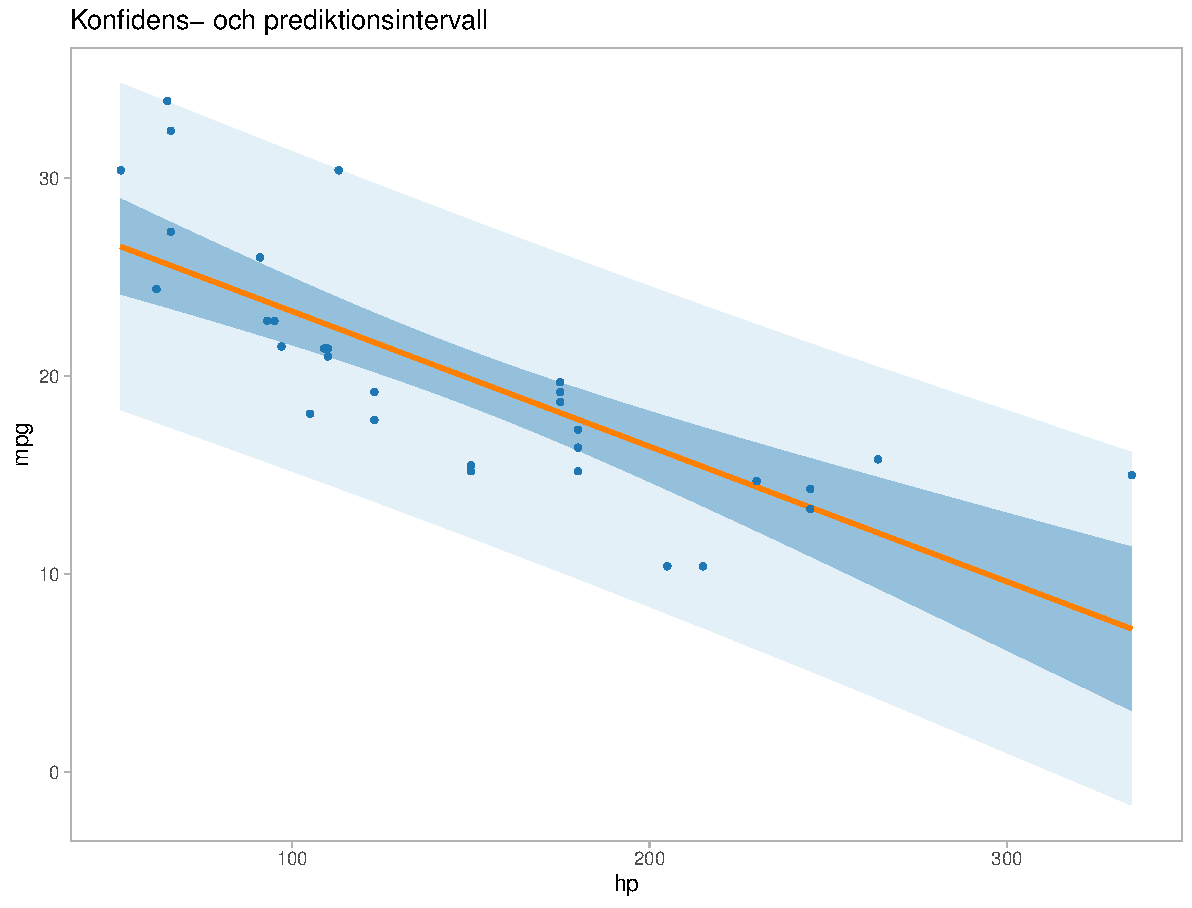
\includegraphics[scale=0.22]{figs/prediction_intervals}
\par\end{center}

\end{frame}

\begin{frame}{\textbf{\textcolor{orange}{Försök, utfall och utfallsrum}}}
\begin{itemize}
\item Vi utför ett \textbf{\textcolor{blue}{försök}} (eng. trial): singlar
ett mynt.
\item Observerar ett \textbf{\textcolor{blue}{utfall}} (eng. outcome): Krona.
\item \textbf{\textcolor{blue}{Utfallsrummet}} är \textbf{\textcolor{orange}{alla
möjliga utfall}} som kan inträffa.
\item Singla slant $S=\left\{ \text{{Krona}},\text{{Klave}}\right\} $.
\item Kasta en tärning:
\end{itemize}
\begin{center}
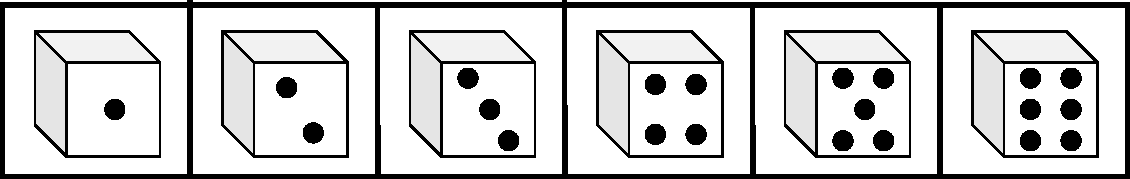
\includegraphics[scale=0.22]{figs/singledice}
\par\end{center}
\begin{itemize}
\item Kasta två tärningar, summera antal prickar.
\end{itemize}
\begin{center}
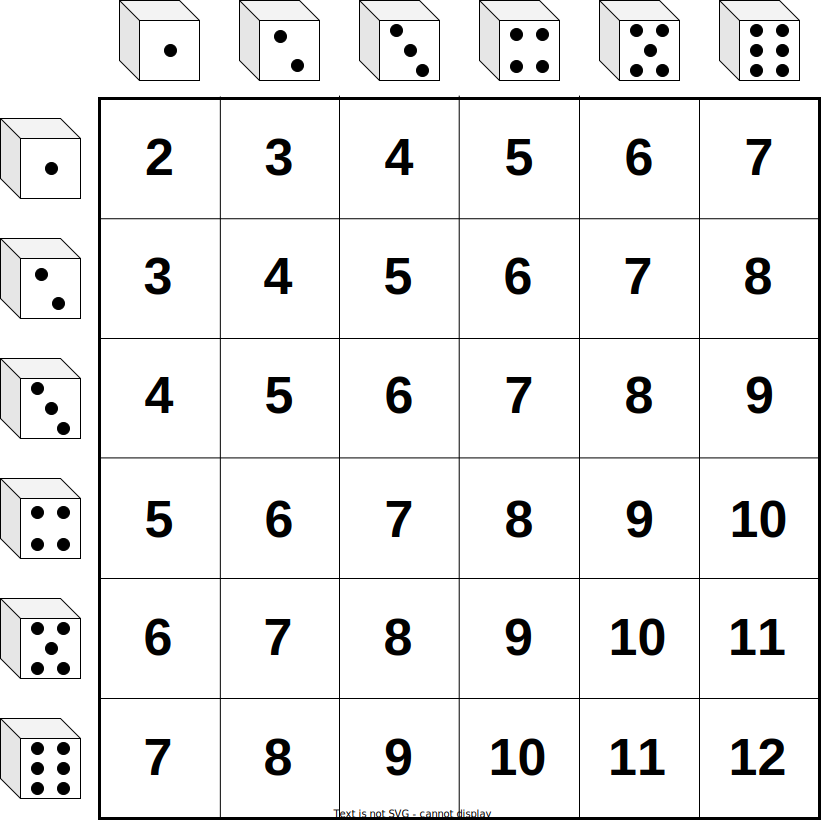
\includegraphics[scale=0.12]{figs/DoubleDice}
\par\end{center}

\end{frame}

\begin{frame}{\textbf{\textcolor{orange}{Händelse - exakt sju prickar med två tärningar}}}
\begin{itemize}
\item En \textbf{\textcolor{blue}{händelse}} är en \textbf{\textcolor{orange}{mängd
av utfall}}.
\item Händelsen A = få exakt 7 prickar med två tärningar.
\[
A=\{(1,6),(2,5),(3,4),(4,3),(5,2),(6,1)\}
\]
\end{itemize}
\begin{center}
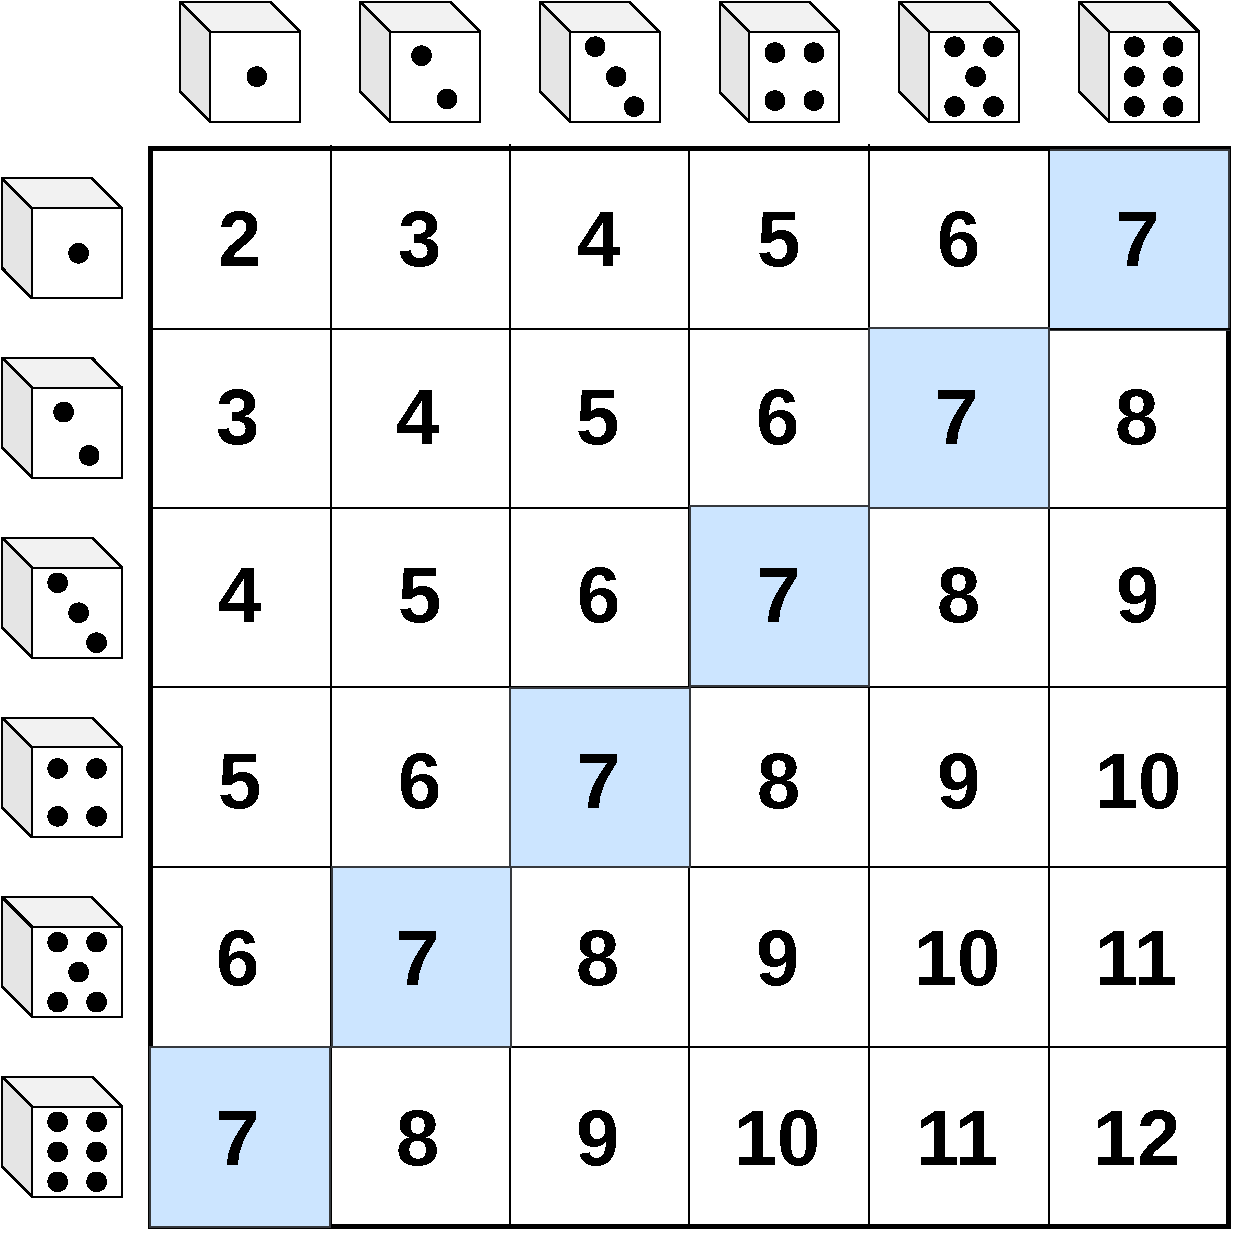
\includegraphics[scale=0.18]{figs/DoubleDiceSeven}
\par\end{center}

\end{frame}

\begin{frame}{\textbf{\textcolor{orange}{Händelse - samma antal prickar på båda
tärningarna}}}
\begin{itemize}
\item Händelsen A = \{få samma antal prickar på båda tärningarna\}
\[
A=\{(1,1),(2,2),(3,3),(4,4),(5,5),(6,6)\}
\]
\end{itemize}
\begin{center}
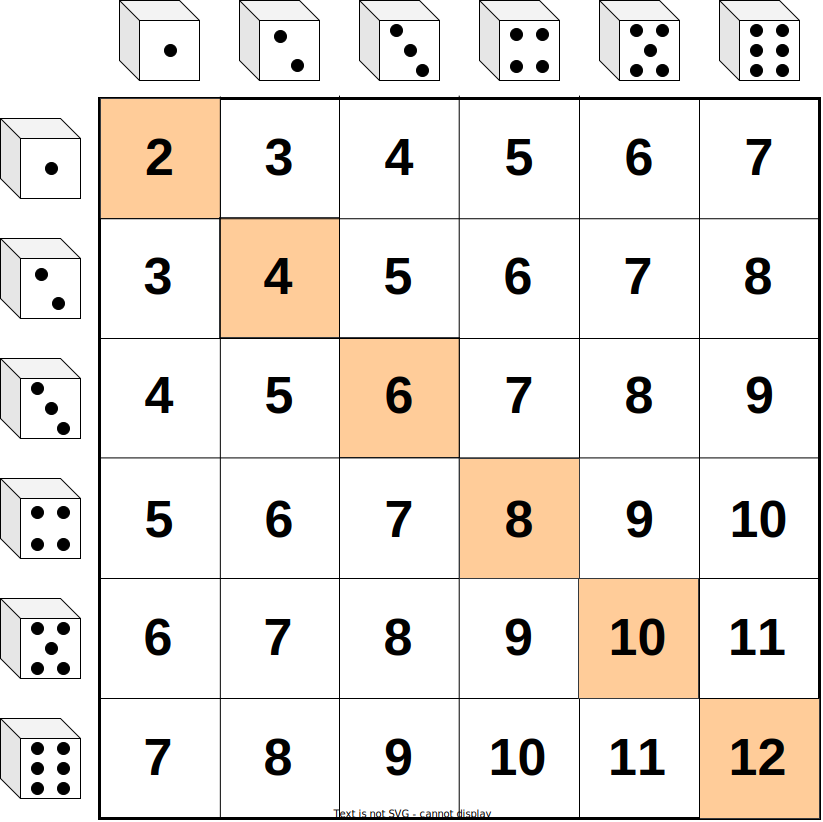
\includegraphics[scale=0.18]{figs/DoubleDiceSame}
\par\end{center}

\end{frame}

\begin{frame}{\textbf{\textcolor{orange}{Tre sannolikhetsbegrepp}}}
\begin{itemize}
\item Vad är \textbf{\textcolor{blue}{sannolikheten}} att få en 6:a med
en tärning?
\begin{itemize}
\item Utfallsrum: $S=\{1,2,3,4,5,6\}$.
\item Händelse: $A=\{6\}$.
\item Sannolikhet: $P(A)$. Måste uppfylla: $0\leq P(A)\leq1$.
\end{itemize}
\end{itemize}
\begin{enumerate}
\item \textbf{\textcolor{blue}{Lika sannolika utfall}} (logisk sannolikhet).
\\
En tärnings fysiska egenskaper → alla sidor är lika sannolika.
\[
P(A)=\frac{\text{antal utfall i }A}{\text{totalt antal möjliga utfall }}=1/6\approx0.1667
\]
\item \textbf{\textcolor{blue}{Empirisk sannolikhet}}: andelen 6:or om jag
kastar tärningen ett \textquotedbl oändligt\textquotedbl{} antal
gånger. 
\[
P(A)=\frac{\text{antal gånger som A inträffar}}{\text{totalt antal försök}}
\]
\item \textbf{\textcolor{blue}{Subjektiva sannolikheter}}. \textbf{Min}
tidigare erfarenhet av tärningskast och \textbf{min} uppfattning om
en tärnings symmetri säger mig att \textbf{min} sannolikhet att få
en 6:a är $1/6\approx0.1667$. 
\end{enumerate}
\end{frame}

\begin{frame}{\textbf{\textcolor{orange}{Stora talens lag - få 6:a med tärning}}}
\begin{center}
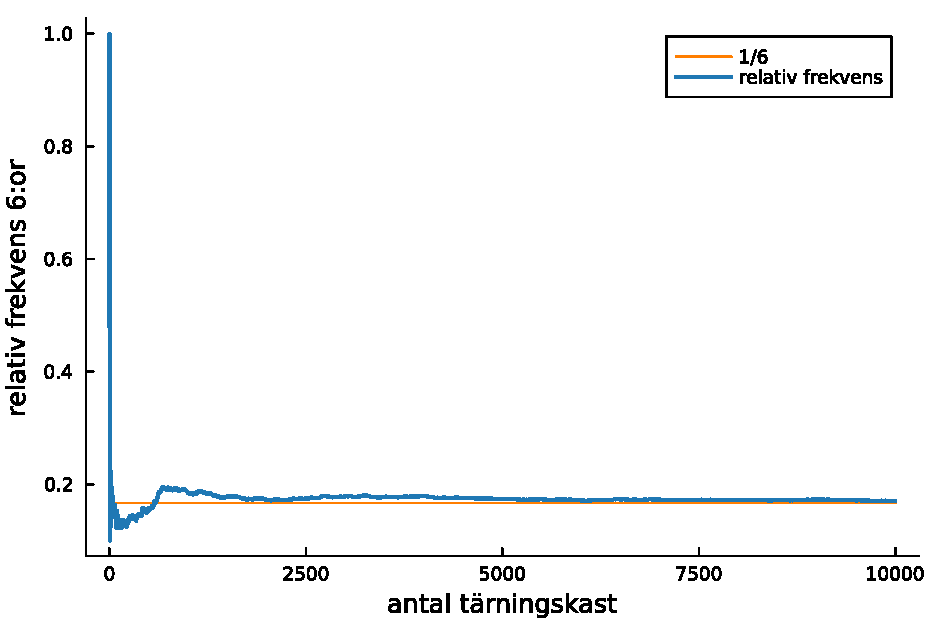
\includegraphics[scale=0.6]{figs/relativfrekvens}
\par\end{center}

\end{frame}

\begin{frame}{\textbf{\textcolor{orange}{Stora talens lag - slantsingling}}}
\begin{center}
\noindent{\fboxrule 1pt\fboxsep 1pt\fcolorbox{orange}{white}{\begin{minipage}[t]{1\columnwidth - 2\fboxsep - 2\fboxrule}%
\begin{center}
\href{https://statisticssu.github.io/SDA1/observable/storatalenslag_bernoulli.html}{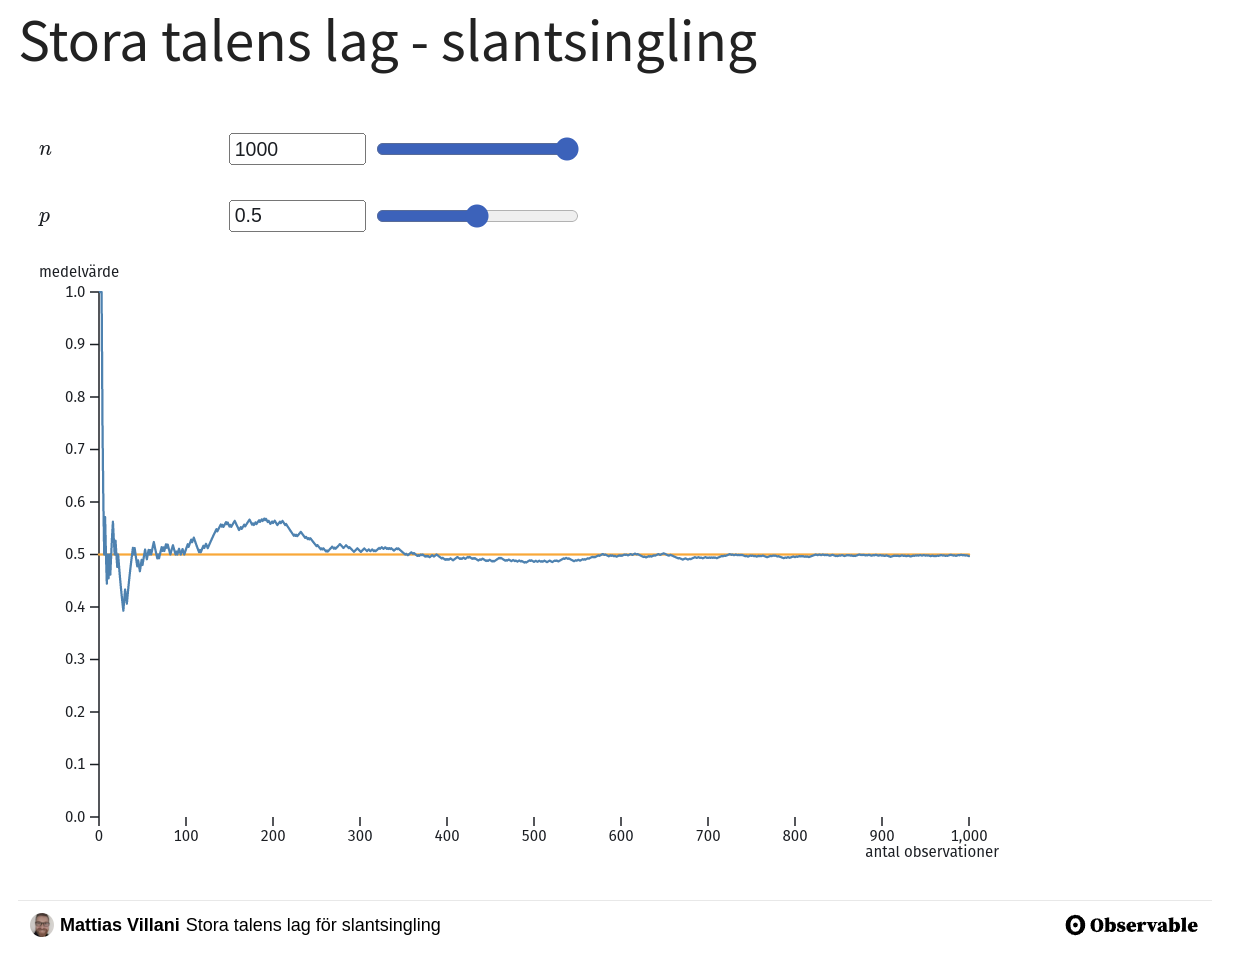
\includegraphics[width=0.9\textwidth]{figs/slantsingling.png}}
\par\end{center}%
\end{minipage}}}
\par\end{center}

\end{frame}

\begin{frame}{\textbf{\textcolor{orange}{Venndiagram}}}
\begin{center}
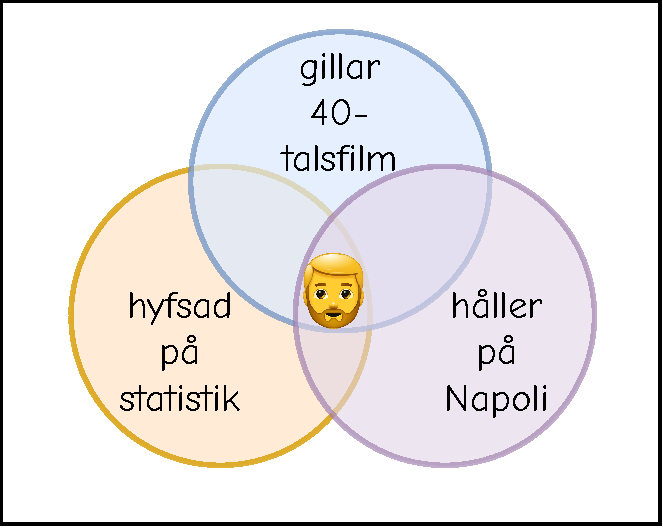
\includegraphics[scale=0.75]{figs/venn_villani}
\par\end{center}

\end{frame}

\begin{frame}{\textbf{\textcolor{orange}{Venndiagram}}}
\begin{center}
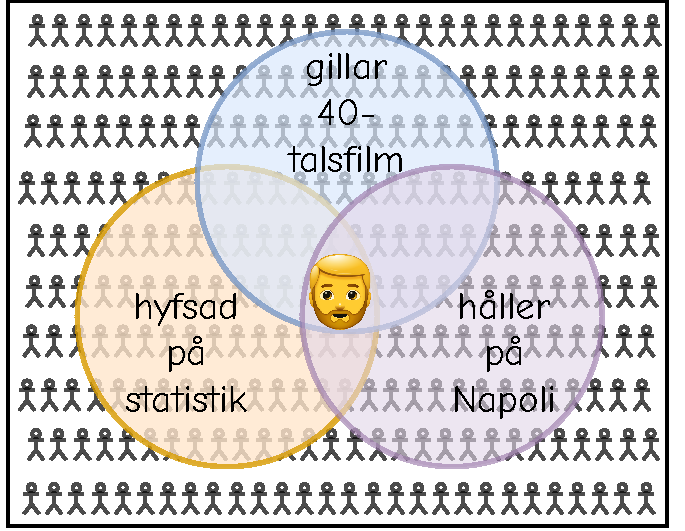
\includegraphics[scale=0.75]{figs/venn_villani_with_people}
\par\end{center}

\end{frame}

\begin{frame}{\textbf{\textcolor{orange}{Händelse - Venndiagram}}}
\begin{itemize}
\item Praktiskt att visualisera händelser i ett \textbf{\textcolor{blue}{Venndiagram}}.
\medskip{}
\item \textbf{\textcolor{blue}{Utfallsrummet}} (allt som kan inträffa) visas
med \textbf{\textcolor{orange}{rektangel}}. \medskip{}
\item \textbf{\textcolor{blue}{Händelser}} ritas som \textbf{\textcolor{orange}{cirklar}},
\textbf{\textcolor{orange}{ellipser}} eller \textbf{\textcolor{orange}{rektanglar}}.\medskip{}
\end{itemize}
\begin{center}
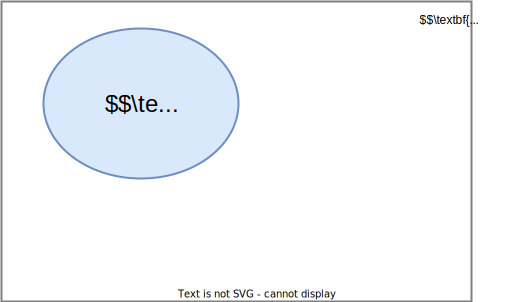
\includegraphics[scale=0.35]{figs/event}\hspace{1cm}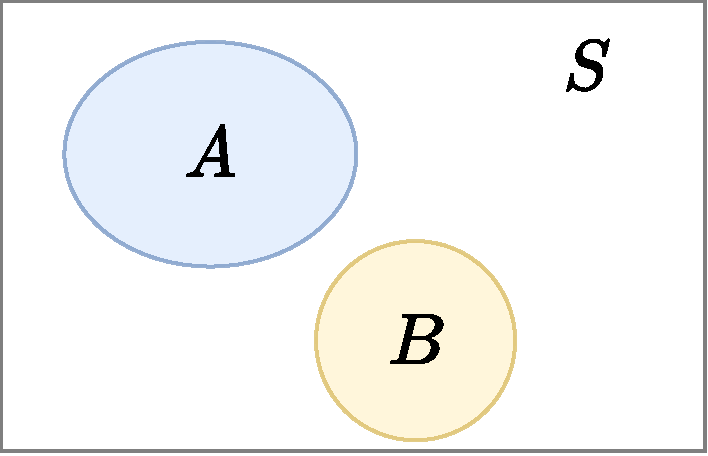
\includegraphics[scale=0.35]{figs/twoevents}
\par\end{center}

\end{frame}

\begin{frame}{\textbf{\textcolor{orange}{Venndiagram - summa sju prickar och samma}}}
\begin{center}
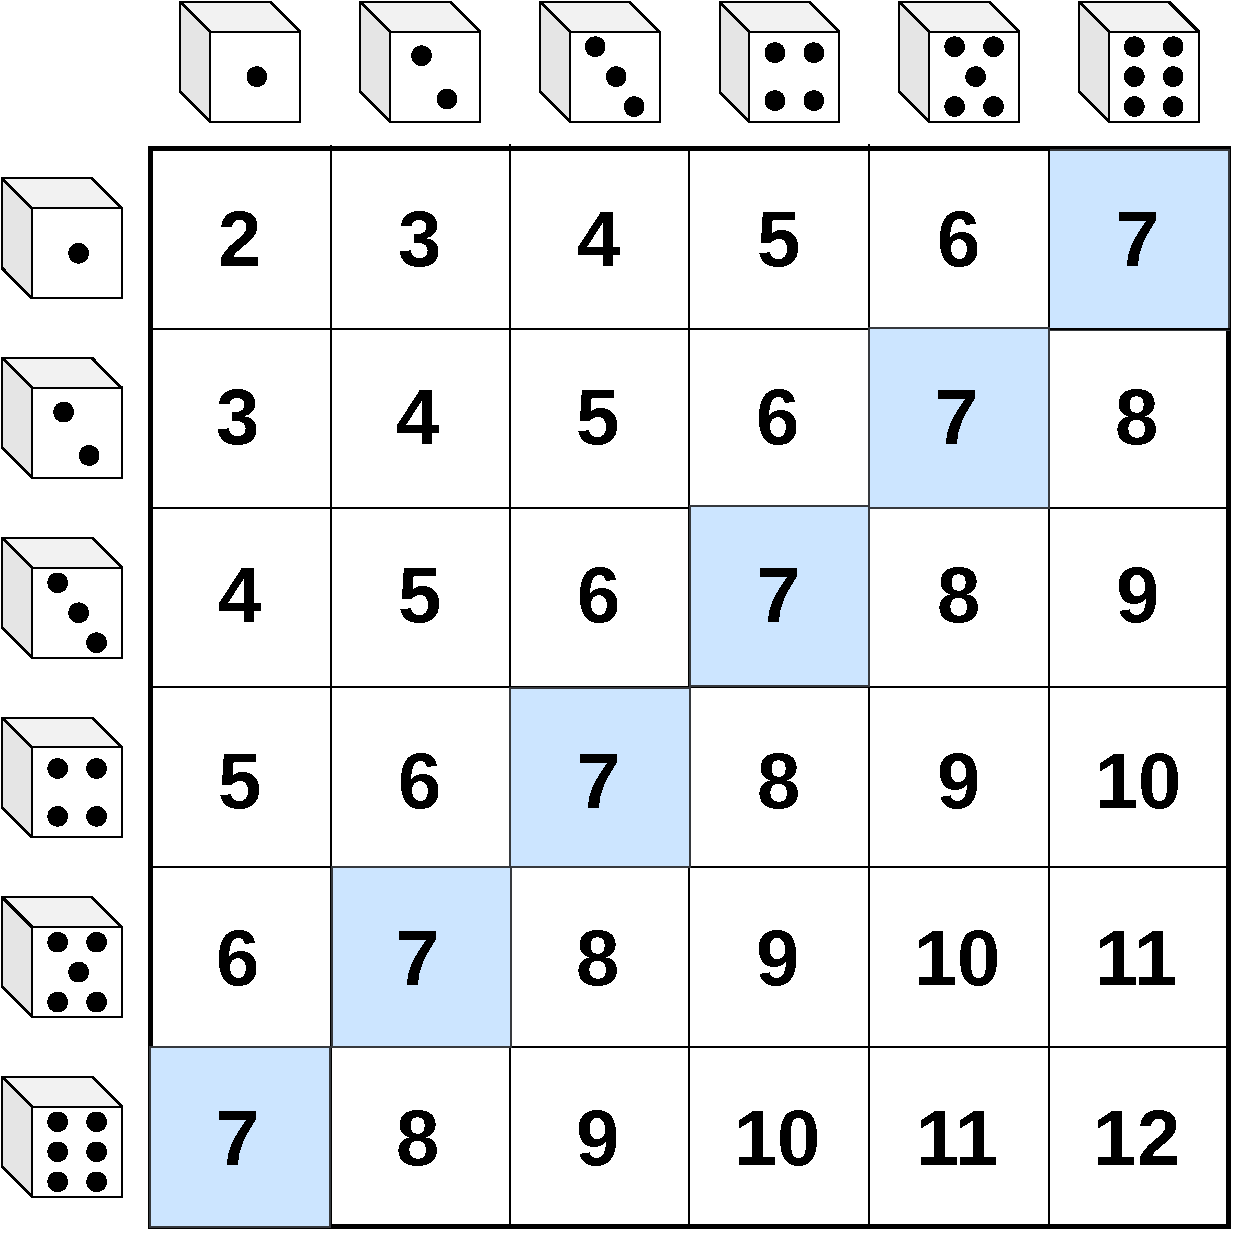
\includegraphics[scale=0.15]{figs/DoubleDiceSeven}\hspace{1cm}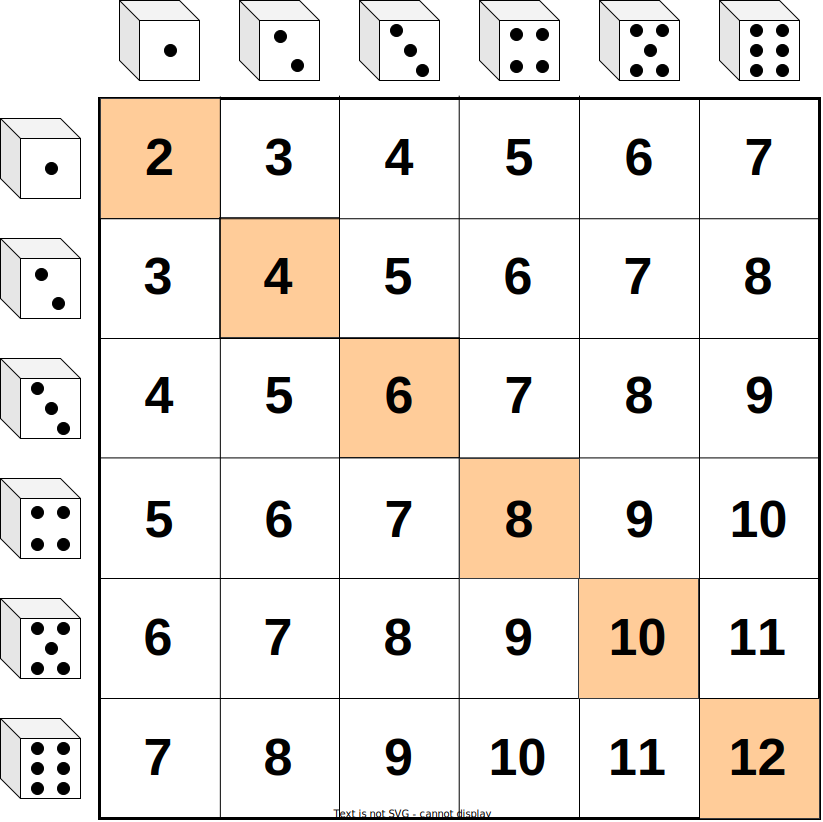
\includegraphics[scale=0.15]{figs/DoubleDiceSame}\vspace{0.5cm}
\\
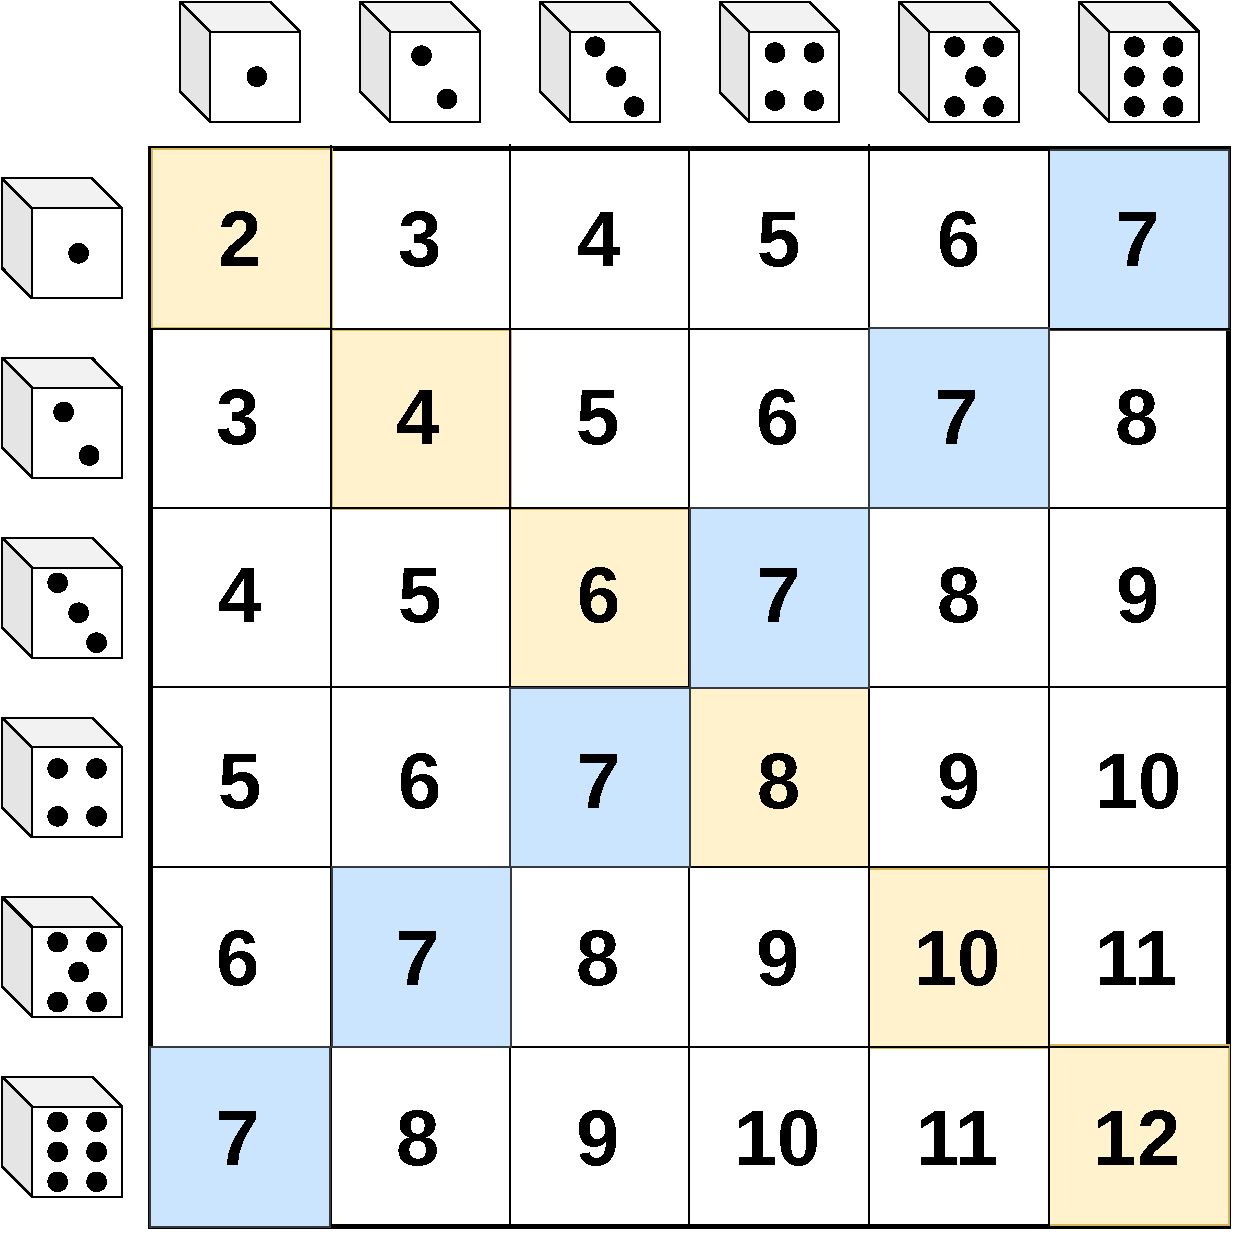
\includegraphics[scale=0.15]{figs/DoubleDiceSevenAndSame}
\par\end{center}

\end{frame}

\begin{frame}{\textbf{\textcolor{orange}{Venndiagram - summa tio prickar och samma}}}
\begin{center}
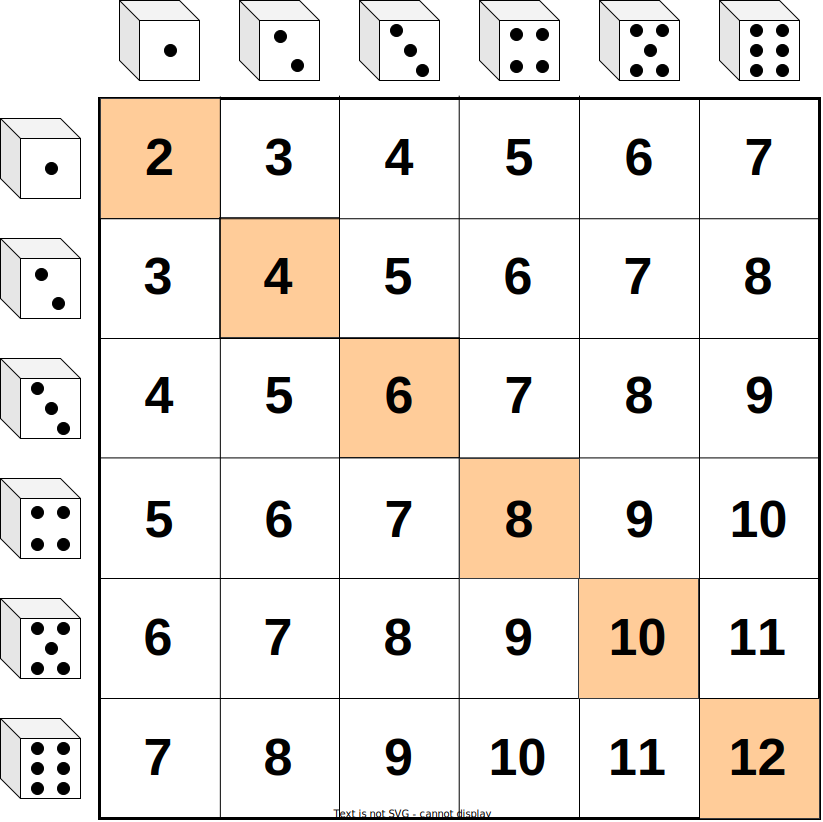
\includegraphics[scale=0.15]{figs/DoubleDiceSame}\hspace{1cm}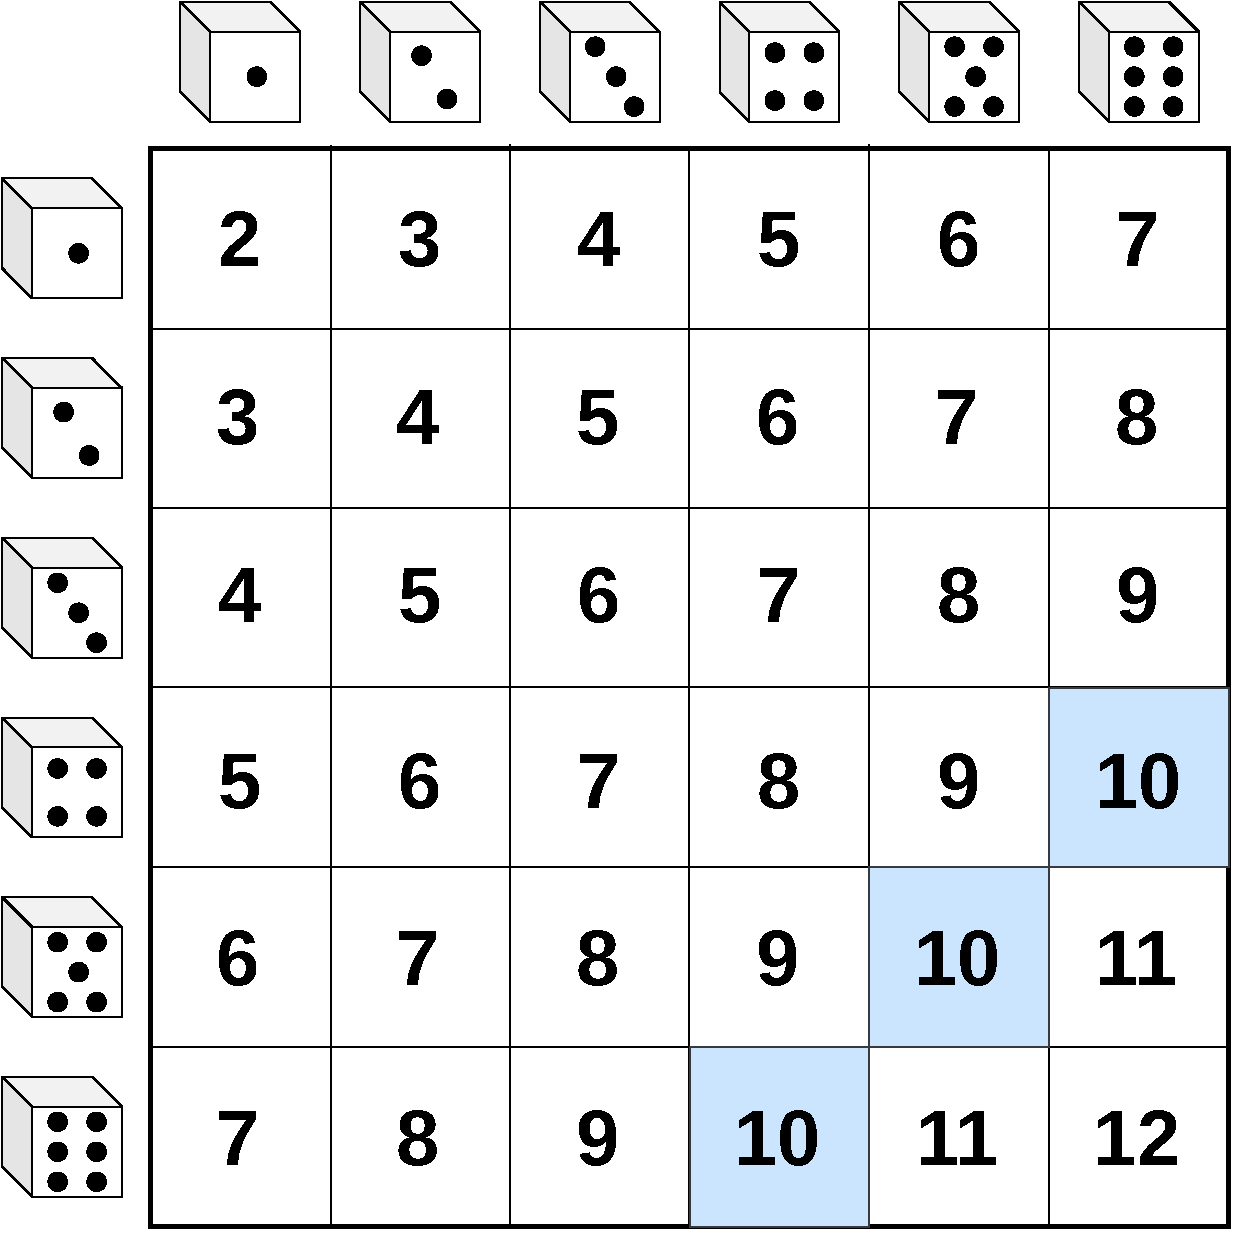
\includegraphics[scale=0.15]{figs/DoubleDiceTen}\vspace{0.5cm}
\\
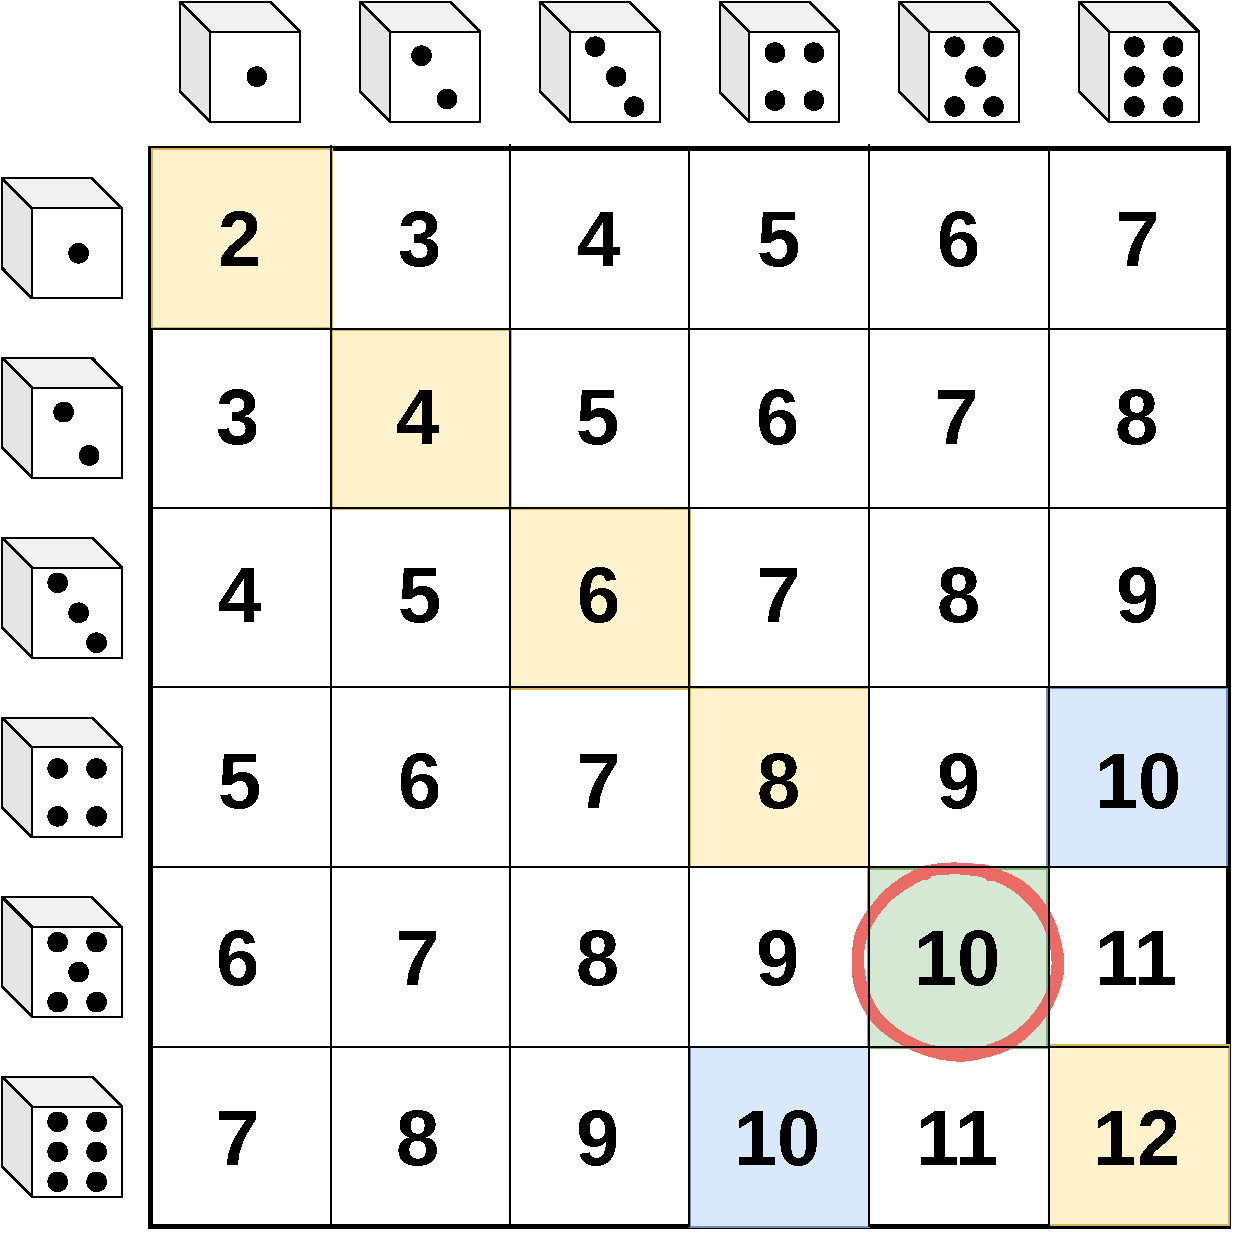
\includegraphics[scale=0.15]{figs/DoubleDiceTenAndSame}\hspace{1cm}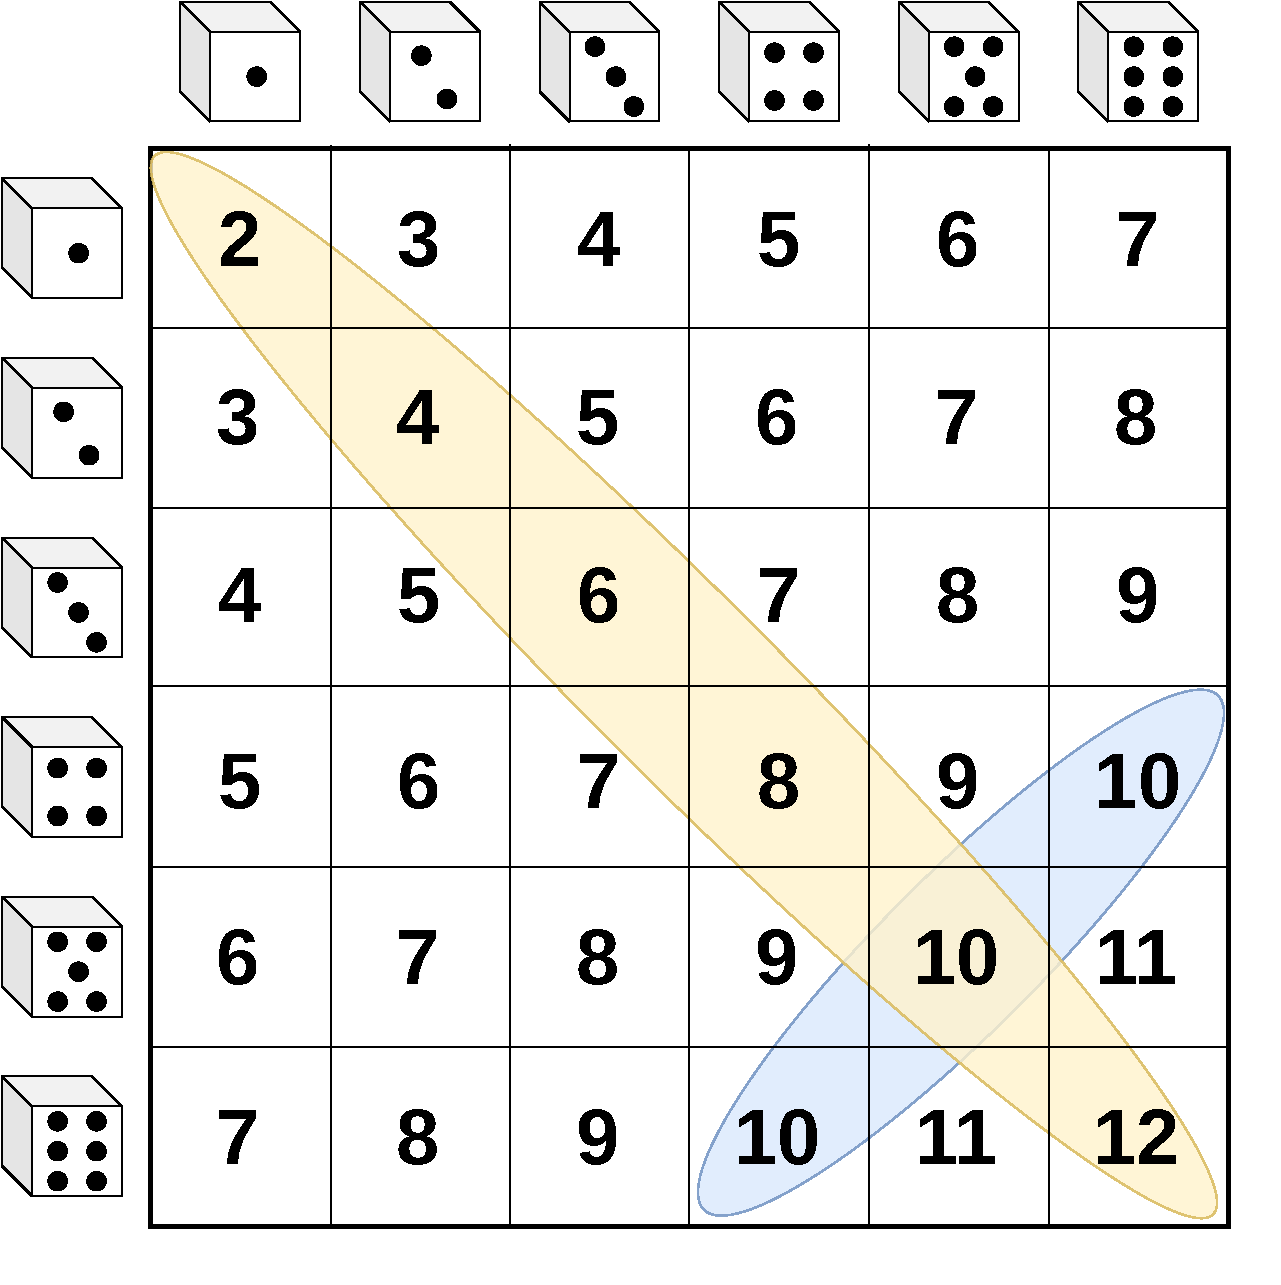
\includegraphics[scale=0.15]{figs/DoubleDiceTenAndSameAbstract}
\par\end{center}

\end{frame}

\begin{frame}{\textbf{\textcolor{orange}{Disjunkta händelser}}}
\begin{center}
\begin{minipage}[t]{0.45\columnwidth}%
\begin{center}
\textbf{\textcolor{blue}{Disjunkta}} händelser\\
inga gemensamma element
\par\end{center}%
\end{minipage}\hspace{0.5cm}%
\begin{minipage}[t]{0.45\columnwidth}%
\begin{center}
\textbf{\textcolor{blue}{Överlappande}} händelser\\
med gemensamma element
\par\end{center}%
\end{minipage}
\par\end{center}

\begin{center}
\begin{minipage}[t]{0.45\columnwidth}%
\begin{center}
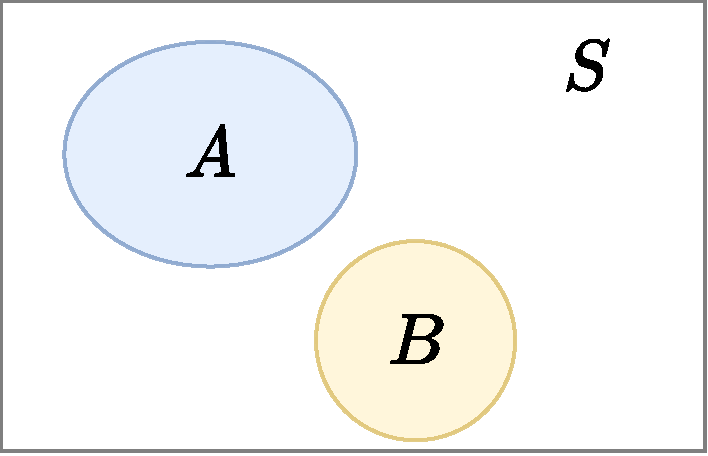
\includegraphics[scale=0.35]{figs/twoevents}
\par\end{center}%
\end{minipage}\hspace{0.5cm}%
\begin{minipage}[t]{0.45\columnwidth}%
\begin{center}
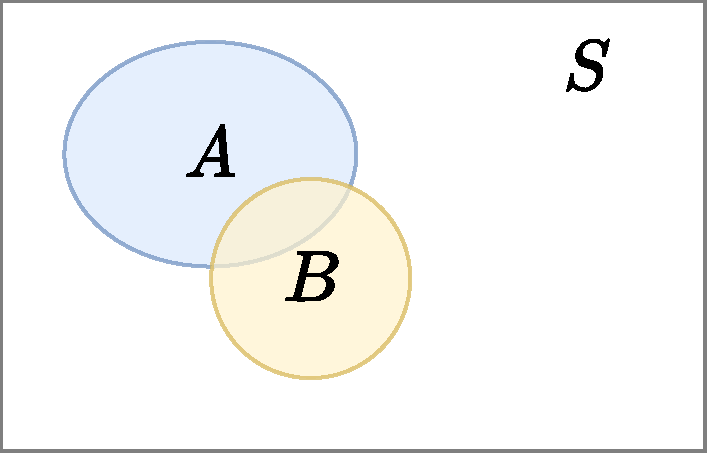
\includegraphics[scale=0.35]{figs/twoeventsoverlap}
\par\end{center}%
\end{minipage}
\par\end{center}

\blfootnote{\tiny \emoji{flag-united-states} Disjunkt = \textcolor{orange} {\textbf{Disjoint}}}
\end{frame}

\begin{frame}{\textbf{\textcolor{orange}{Komplementshändelsen}}}
\begin{itemize}
\item \textbf{\textcolor{blue}{Komplementet}} till A inträffar när \textbf{\textcolor{orange}{A
inte inträffar}}.  \smallskip{}
 
\item Vi skriver $\mathbf{A}^{c}$ där $c$ står för engelskans \textbf{\textcolor{orange}{C}}omplement.\smallskip{}
\end{itemize}
\begin{center}
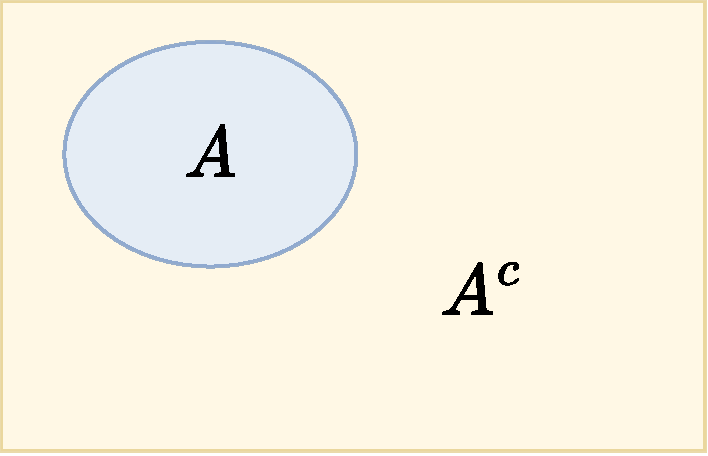
\includegraphics[scale=0.25]{figs/complement}
\par\end{center}

\vspace{-0.35cm}

\begin{minipage}[t]{0.83\columnwidth}%
\begin{itemize}
\item {\footnotesize{}Tärningar}{\footnotesize\par}
\begin{itemize}
\item {\footnotesize{}$\mathbf{A}$ = \{udda antal prickar på tärning\}
= \{1,3,5\}.}{\footnotesize\par}
\item {\footnotesize{}$\mathbf{A}^{c}$ = \{jämnt antal prickar på tärning\}
= \{2,4,6\}.\medskip{}
}{\footnotesize\par}
\end{itemize}
\item {\footnotesize{}Inflation}{\footnotesize\par}
\begin{itemize}
\item {\footnotesize{}$\mathbf{A}$ = \{inflationen nästa månad $\leq2$\}.}{\footnotesize\par}
\item {\footnotesize{}$\mathbf{A}^{c}$ = \{inflationen nästa månad $>2$\}.\medskip{}
}{\footnotesize\par}
\end{itemize}
\item {\footnotesize{}Mjukvarubuggar}{\footnotesize\par}
\begin{itemize}
\item {\footnotesize{}$\mathbf{A}$ = \{ingen bugg i programvaran\}.}{\footnotesize\par}
\item {\footnotesize{}$\mathbf{A}^{c}$ = \{minst en bugg\} = \{1 bugg,
2 buggar, ...\}}{\footnotesize\par}
\end{itemize}
\end{itemize}
%
\end{minipage}%
\begin{minipage}[t][1\totalheight][c]{0.15\columnwidth}%
\begin{center}
\vspace{0.4cm}

\includegraphics[scale=0.03]{figs/flaticons/dicered}\vspace{0.5cm}
\par\end{center}
\begin{center}
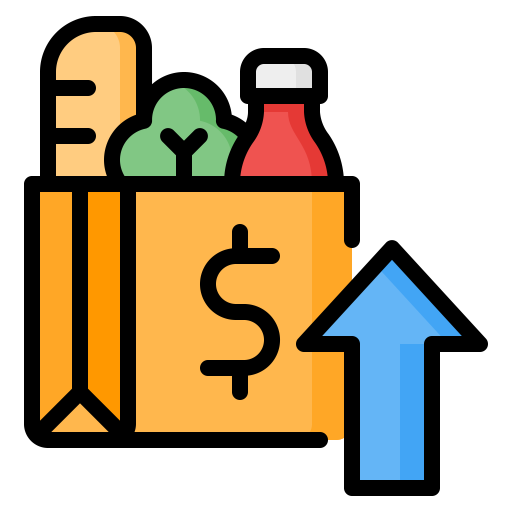
\includegraphics[scale=0.07]{figs/flaticons/grocery}\vspace{0.3cm}
\par\end{center}
\begin{center}

\includegraphics[scale=0.04]{figs/flaticons/bug}
\par\end{center}%
\end{minipage}

\end{frame}

\begin{frame}{\textbf{\textcolor{orange}{Snitthändelsen}}}
\begin{itemize}
\item \textbf{\textcolor{blue}{Snitthändelsen}} är händelsen där \textbf{\textcolor{blue}{både
A och B}} inträffar.\smallskip{}
 
\item Vi skriver $\textcolor{orange}{\mathbf{A\text{ och }B}}$ eller $\textcolor{orange}{\mathbf{\mathbf{A}\cap\mathbf{B}}}$.\hspace{1.9cm}
\tiny \emoji{flag-united-states} Snitt = \textcolor{orange} {\textbf{Intersection}}\smallskip{}
\end{itemize}
\begin{center}
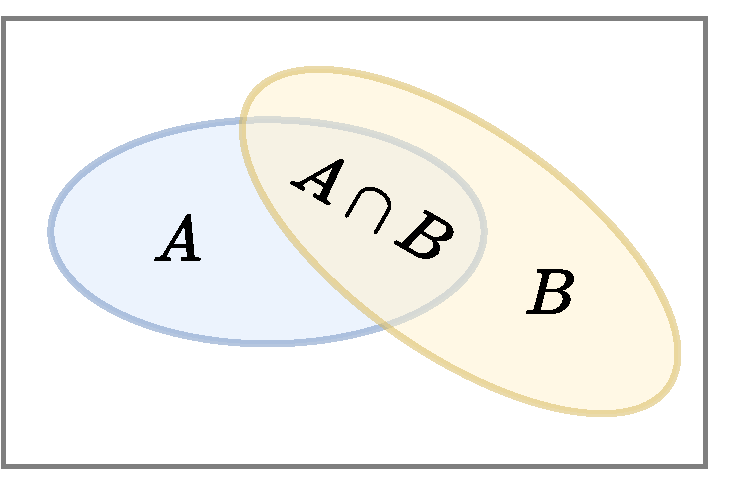
\includegraphics[scale=0.25]{figs/intersection}
\par\end{center}
\begin{itemize}
\item Två tärningar:
\begin{itemize}
\item {\footnotesize{}$\mathbf{A}$ = \{samma prickar på båda tärningar\}}{\footnotesize\par}
\item {\footnotesize{}$\mathbf{B}$ = \{totalt 10 prickar\}}{\footnotesize\par}
\item {\footnotesize{}$\mathbf{A}\cap\mathbf{B}$ = \{5:a på båda tärningar\}}{\footnotesize\par}
\end{itemize}
\item {\footnotesize{}Lågkonjunktur {\large \emoji{anxious-face-with-sweat}}}\smallskip{}

\begin{itemize}
\item {\footnotesize{}$\mathbf{A}$ = \{BNP-tillväxt kvartal 1 $<0$\}}{\footnotesize\par}
\item {\footnotesize{}$\mathbf{B}$ = \{BNP-tillväxt kvartal 2 $<0$\}}{\footnotesize\par}
\item {\footnotesize{}$\mathbf{A}\cap\mathbf{B}$ = \{Negativ BNP-tillväxt
två kvartal i rad\}\bigskip{}
}{\footnotesize\par}
\end{itemize}
\item {\footnotesize{}Disjunkta händelsers snitt är den }\textbf{\textcolor{blue}{\footnotesize{}tomma
mängden}}{\footnotesize{} $\emptyset$ 
\[
\mathbf{A}\text{ och }\textbf{\ensuremath{\mathbf{B}}}\text{ disjunkta }\quad\Longleftrightarrow\quad\mathbf{A}\cap\textbf{\ensuremath{\mathbf{B}}}=\mathbf{\emptyset}
\]
}{\footnotesize\par}
\end{itemize}
\end{frame}

\begin{frame}{\textbf{\textcolor{orange}{Unionhändelsen}}}
\begin{itemize}
\item \textbf{\textcolor{blue}{Unionhändelsen}} är händelsen där\textbf{\textcolor{blue}{{}
A och/eller B}} inträffar.\smallskip{}
\item \textbf{\textcolor{blue}{Minst en}} av händelserna inträffar.
\end{itemize}
\begin{center}
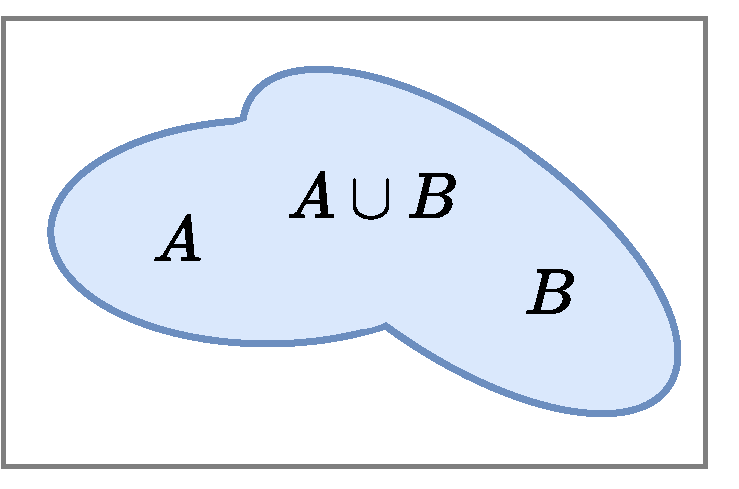
\includegraphics[scale=0.3]{figs/union}
\par\end{center}
\begin{itemize}
\item Universitetstudier {\footnotesize{}{\large \emoji{woman-student}}}\smallskip{}

\begin{itemize}
\item {\footnotesize{}$\mathbf{A}$ = \{Kommer in på kurs på betyg\}}\smallskip{}
\item {\footnotesize{}$\mathbf{B}$ = \{Kommer in på kurs på högskoleprov\}}\smallskip{}
\item {\footnotesize{}$\mathbf{A\cup\textbf{B}}$ = \{Kommer in på kurs\}}{\footnotesize\par}
\end{itemize}
\end{itemize}
\end{frame}

\begin{frame}{\textbf{\textcolor{orange}{Formell sannolikhet}}}

\footnotesize
\begin{tcolorbox}[colback=verylightgray]

\textcolor{blue}{\textbf{Sannolikheten}} $P(A)$ för händelse $A$ på utfallsrummet $S$
\begin{enumerate}
	\item $0\leq P(A)\leq1$
	\item $P(S)=1$
    \item $P(A^c)=1-P(A)$
	\item $P(A\cup B)=P(A)+P(B)$ om $A$ och $B$ är \textbf{disjunkta}
    \item $P(A \cap B) = P(A)\cdot P(B)$ om $A$ och $B$ är \textbf{oberoende}
\end{enumerate}

\end{tcolorbox}
\normalsize

\medskip{}

\begin{enumerate}
\item {\small{}En sannolikhet är ett tal mellan 0 och 1.\smallskip{}
}{\small\par}
\item {\small{}Sannolikheten för en }\textbf{\textcolor{blue}{\small{}säker
händelse}}{\small{} är 1.\smallskip{}
}{\small\par}
\item {\small{}Sannolikheten att en händelse }\textbf{\textcolor{blue}{\small{}inte}}{\small{}
inträffar är 1 minus sannolikheten för händelsen.\smallskip{}
}{\small\par}
\item {\small{}Sannolikheten att }\textbf{\textcolor{blue}{\small{}åtminstone
en}}{\small{} av två händelser som }\textbf{\textcolor{blue}{\small{}inte
kan inträffa samtidigt}}{\small{} är summan av händelsernas sannolikheter.\smallskip{}
}{\small\par}
\item {\small{}Sannolikheten att två oberoende händelser }\textbf{\textcolor{blue}{\small{}båda}}{\small{}
inträffar är produkten av händelsernas sannolikheter.}{\small\par}
\end{enumerate}
\end{frame}

\begin{frame}{\textbf{\textcolor{orange}{Komplementsregeln}}}
\begin{itemize}
\item $A$ och $A^{c}$ är \textbf{\textcolor{blue}{disjunkta}}. Kan inte
inträffa samtidigt.
\item Någon av $A$ eller $A^{c}$ \emph{måste} inträffa.
\[
P(A)+P(A^{c})=1
\]
\end{itemize}
\begin{tcolorbox}[colback=verylightgray]
\textcolor{blue}{\textbf{Komplementsregeln}}
$$P(A^{c})=1-P(A)$$
\end{tcolorbox}
\begin{center}
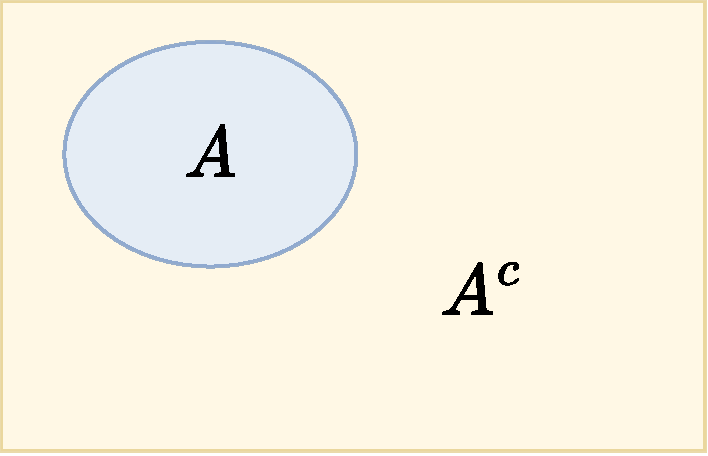
\includegraphics[scale=0.25]{figs/complement}
\par\end{center}
\begin{itemize}
\item {\footnotesize{}$\mathbf{A}$ = \{ingen bugg i koden\}.}{\footnotesize\par}
\item {\footnotesize{}$\mathbf{A}^{c}$ = \{}\textbf{\textcolor{orange}{\footnotesize{}åtminstone
en}}{\footnotesize{} bugg i koden\} = \{1 bugg, 2 buggar, ...\}}{\footnotesize\par}
\item {\small{}$P(\left\{ \text{minst en bugg i koden}\right\} )=1-P(\text{\ensuremath{\left\{  \text{ingen bugg i koden}\right\} } })$.}{\small\par}
\end{itemize}
\end{frame}

\begin{frame}{\textbf{\textcolor{orange}{Den allmänna additionsregeln}}}
\begin{itemize}
\item \textbf{\textcolor{blue}{Additionsregeln}}: Om $A$ och $B$ är \textbf{\textcolor{orange}{disjunkta}}:
\[
P(A\cup B)=P(A)+P(B)
\]
\end{itemize}
\begin{tcolorbox}[colback=verylightgray]
\textcolor{blue}{\textbf{Allmänna additionsregeln} (även överlappande händelser)}
$$P(A\cup B)=P(A)+P(B)-P(A\cap B)$$
\end{tcolorbox}
\begin{itemize}
\item Måste dra bort snittet $A\cap B$ för det räknas två ggr.
\end{itemize}
\begin{center}
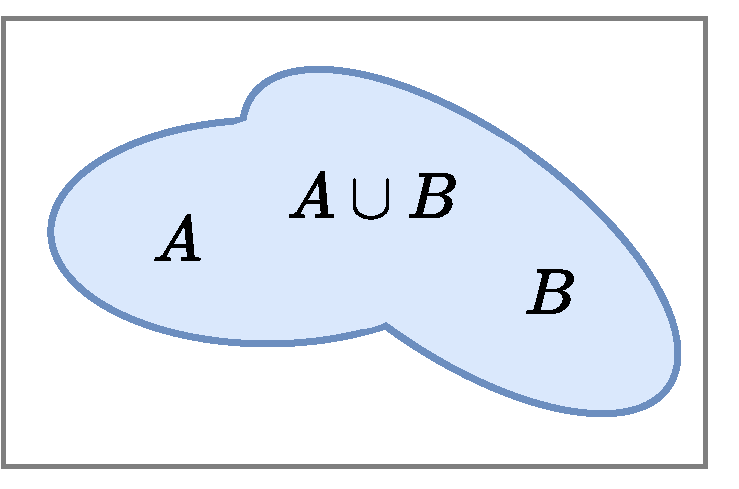
\includegraphics[scale=0.4]{figs/union}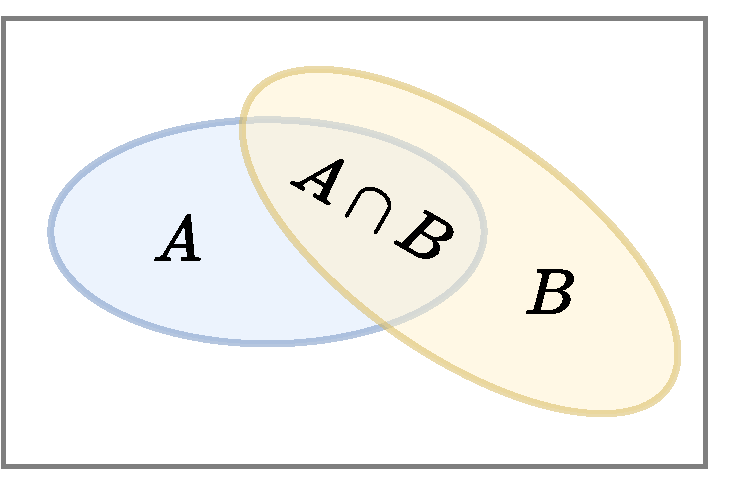
\includegraphics[scale=0.4]{figs/intersection}
\par\end{center}

\end{frame}

\begin{frame}{\textbf{\textcolor{orange}{Röst på socialdemokraterna }}\emoji{rose}
\textbf{\textcolor{orange}{additionsregeln}}}
 
\begin{itemize}
\item \textbf{$\mathbf{R}$} = person röstar \emoji{rose} i riksdagsvalet.
$P(\mathbf{R})=0.2$
\item $\mathbf{K}$ = person röstar \emoji{rose} i kommunalvalet. $P(\mathbf{K})=0.3$
\item Personen röstar på \emoji{rose} in båda valen: $P(\text{\ensuremath{\mathbf{R}} \ensuremath{\cap} \ensuremath{\mathbf{K}}})=0.1$
\item Röstar \emoji{rose} i åtminstone ett av valen? Additionsregeln:
\[
P(\text{\ensuremath{\mathbf{R}} \ensuremath{\cup} \ensuremath{\mathbf{K}}})=0.2+0.3-0.1=0.4
\]
\item Röstar inte på \emoji{rose} i något av valen?
\[
P(\mathbf{R}^{c}\cap\mathbf{K}^{c})=P((\text{\ensuremath{\mathbf{R}} \ensuremath{\cup} \ensuremath{\mathbf{K}}})^{c})=1-P(\text{\ensuremath{\mathbf{R}} \ensuremath{\cup} \ensuremath{\mathbf{K}}})=1-0.4=0.6
\]
\end{itemize}
\begin{center}
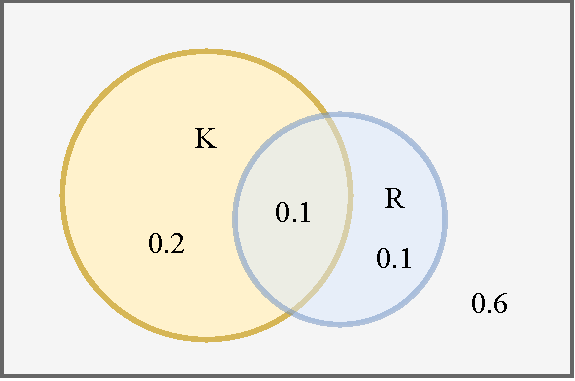
\includegraphics[scale=0.3]{figs/SocialdemokratVenn}
\par\end{center}

\end{frame}

\begin{frame}{\textbf{\textcolor{orange}{Multiplikationssregeln för oberoende händelser}}}
\begin{itemize}
\item Händelserna $A$ och $B$ är \textbf{\textcolor{blue}{oberoende}}
om vetskapen att $B$ har inträffat \textbf{\textcolor{orange}{inte
påverkar}} sannolikheten för $A$. Och vice versa.\medskip{}
\item Test: kommer sannolikheten för $A$ förändras om man får veta att
\textbf{$B$} har inträffat? Om inte, så är $A$ och $B$ oberoende.\textbf{\bigskip{}
}
\end{itemize}
\begin{tcolorbox}[colback=verylightgray]
\textcolor{blue}{\textbf{Multiplikationsregeln}}. För \textcolor{orange}{\textbf{oberoende}} händelser $A$ och $B$
$$P(A\cap B)=P(A)\cdot P(B)$$
\end{tcolorbox}\medskip{}

\begin{itemize}
\item Hur beräknar man sannolikheten för snittet $A\cap B$ för händelser
som \textbf{inte} är oberoende? Stay tuned, kommer i F12. 
\includegraphics[scale=0.2]{figs/face-with-peeking-hand}\medskip{}
\end{itemize}
\end{frame}

\begin{frame}{\textbf{\textcolor{orange}{Multiplikationsregeln för oberoende händelser}}}
 
\begin{itemize}
\item Vad är sannolikheten att få 2 st krona i rad vid slantsingling?
\[
0.5\cdot0.5=0.5^{2}=0.25
\]
\item Vad är sannolikheten att få 5 st krona i rad vid slantsingling?
\[
0.5\cdot0.5\cdot0.5\cdot0.5\cdot0.5=0.5^{5}=0.03125
\]
\item 1\% risk att streaming laggar under en kväll. Oberoende kvällar. 
\[
P(\text{ingen lagg hela veckan)}=(1-0.01)^{7}=0.99^{7}\approx0.932.
\]
\smallskip{}
\item Sannolikheten att dra två klöver \includegraphics[scale=0.25]{figs/flaticons/clubs}
ur en blandad kortlek?{\footnotesize{}
\[
P(\text{1:a kortet klöver)}=\frac{13}{52}=\frac{1}{4}
\]
\[
P(\text{2:a kortet klöver \textbf{givet} 1:a kortet klöver)}=\frac{12}{51}
\]
\[
P(\text{2:a kortet klöver \textbf{givet} 1:a kortet \textbf{inte} klöver)}=\frac{13}{51}
\]
}{\footnotesize\par}
\item $A=$$\{$\includegraphics[scale=0.25]{figs/flaticons/clubs}\textrm{
på 1:a}\} och $B=$$\{$\includegraphics[scale=0.25]{figs/flaticons/clubs}\textrm{
på 2:a}\} är \textbf{inte} oberoende.
\end{itemize}
\end{frame}

\begin{frame}{\textbf{\textcolor{orange}{Röst på socialdemokraterna }}\emoji{rose}
\textbf{\textcolor{orange}{multiplikationsregeln}}}
 
\begin{itemize}
\item \textbf{$\mathbf{R}$} = person röstar \emoji{rose} i riksdagsvalet.
$P(\mathbf{R})=0.2$
\item $\mathbf{K}$ = person röstar \emoji{rose} i kommunalvalet. $P(\mathbf{K})=0.3$
\item Personen röstar på \emoji{rose} in båda valen: $P(\text{\ensuremath{\mathbf{R}} \ensuremath{\cap} \ensuremath{\mathbf{K}}})=0.1$
\item Är händelserna \textbf{$\mathbf{R}$} och $\mathbf{K}$ \textbf{\textcolor{blue}{oberoende}}?
Vi måste undersöka om 
\[
P(\text{\ensuremath{\mathbf{R}} \ensuremath{\cap} \ensuremath{\mathbf{K}}})=P(\mathbf{R})\cdot P(\mathbf{K})
\]
\item Händelserna är \textbf{inte} oberoende:
\[
P(\mathbf{R})\cdot P(\mathbf{K})=0.2\cdot0.3\neq0.1=P(\text{\ensuremath{\mathbf{R}} \ensuremath{\cap} \ensuremath{\mathbf{K}}})
\]
\item Att hen röstat på \emoji{rose} i kommunalvalet ger information om
vad hen röstat på i riksdagsvalet.
\item \textbf{\textcolor{blue}{Betingad sannolikhet}} för $\mathbf{R}$
\textbf{\textcolor{blue}{givet}} $\mathbf{K}$ är sann: $0.333$ (se
F13).
\item $P(\mathbf{R})$ ökar från $0.2$ till $0.333$ när vi vet att $\mathbf{K}$
är sann.
\end{itemize}
\end{frame}

\begin{frame}{\textbf{\textcolor{orange}{Kombinatorik}}}
\begin{itemize}
\item Dataset 1: \textbf{\textcolor{orange}{med ordning}}: $\text{Krona},\text{Klave},\text{Klave},\text{Krona},\text{Krona}$.
\item Dataset 2: \textbf{\textcolor{orange}{utan ordning}}: 3 st Krona och
2 st Klave.
\item Är det lika sannolikt att observera Dataset 1 som Dataset 2?\medskip{}
\item \textbf{\textcolor{blue}{Kombinatorik}}: räknar antal sätt/kombinationer.\smallskip{}
\item \textbf{\textcolor{blue}{Fakultetet}} (eng. factorial). Utläses som
n-fakultet. 
\[
n!=n(n-1)(n-2)\cdots2\cdot1
\]
\end{itemize}
\begin{tcolorbox}[width=0.85\hsize, tab2, tabularx={c|c|c}, boxrule=0.5pt, 
title = Hur många sätt att välja $k$ element bland $n$ element?]  & \vspace{0.0cm} med återläggning     & utan återläggning      \\\hline med ordning   & $n^k$  & $\,_nP_k = \frac{n!}{(n-k)!}$                             \\\hline utan ordning   & ej på kurs & $ \,_nC_k = \frac{n!}{(n-k)!k!}$   \end{tcolorbox}
\end{frame}

\begin{frame}{\textbf{\textcolor{orange}{Med återläggning, med hänsyn till ordning}}}
\begin{center}
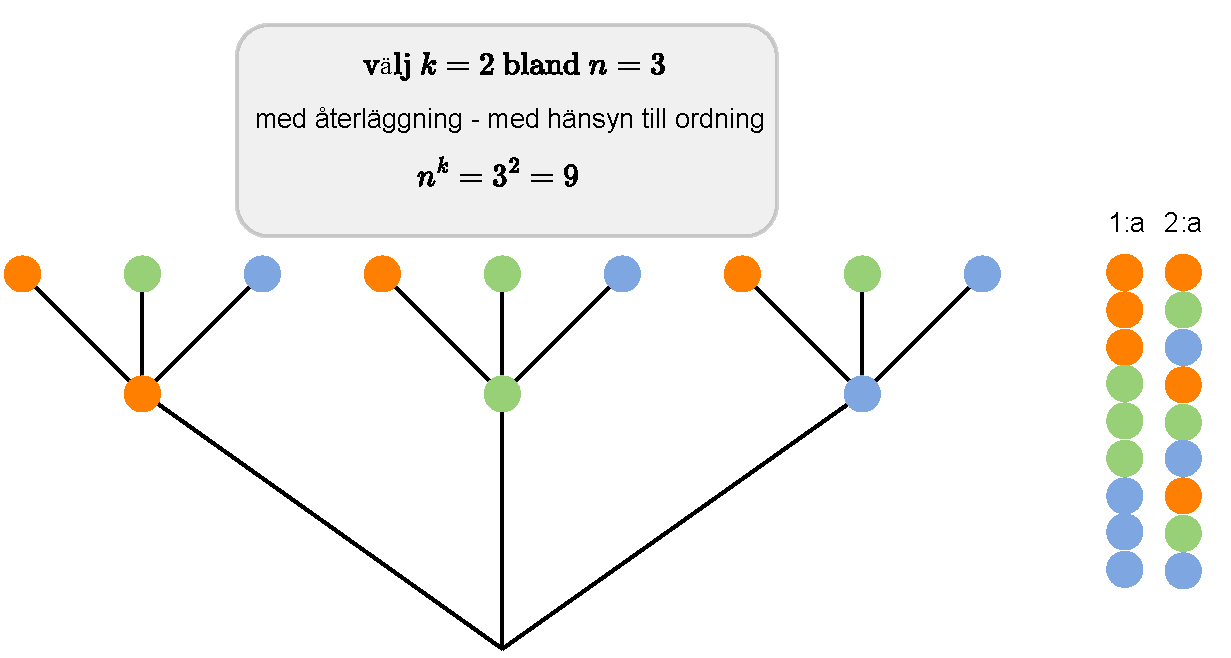
\includegraphics[scale=0.45]{figs/BallsNoReplaceWithOrder}
\par\end{center}

\end{frame}

\begin{frame}{\textbf{\textcolor{orange}{Utan återläggning, med hänsyn till ordning}}}
\begin{center}
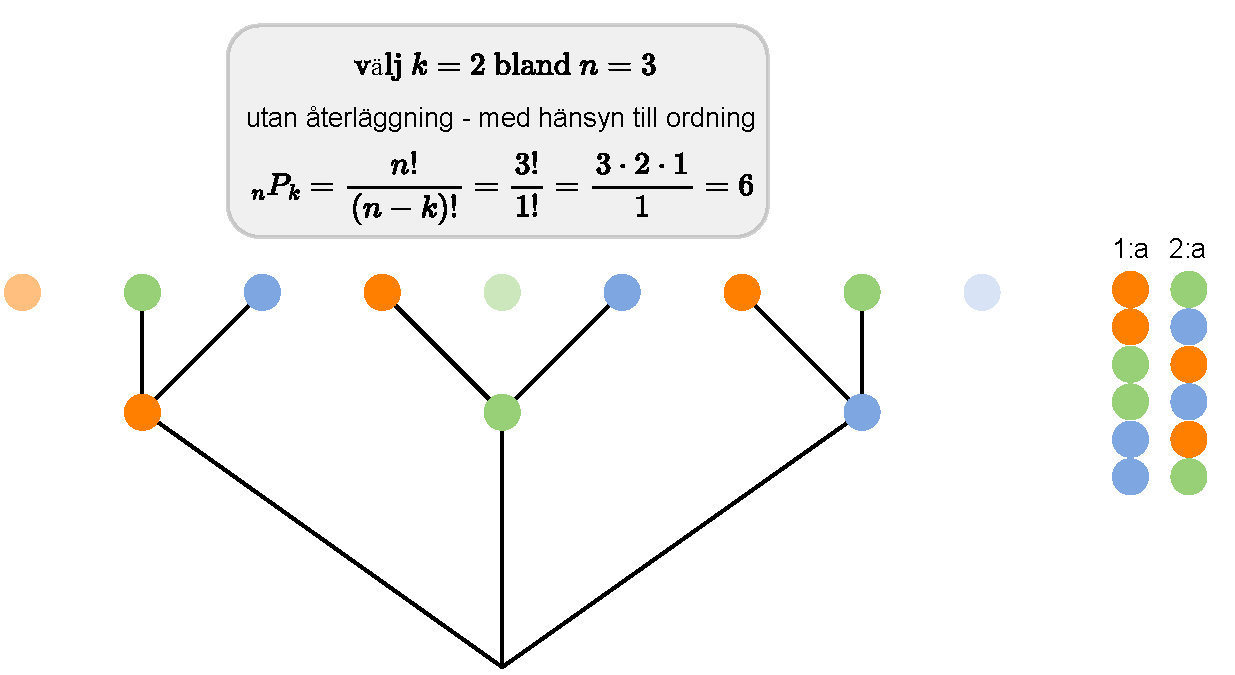
\includegraphics[scale=0.45]{figs/BallsNoReplaceWithOrdering}
\par\end{center}

\end{frame}

\begin{frame}{\textbf{\textcolor{orange}{Utan återläggning, utan hänsyn till ordning}}}
\begin{center}
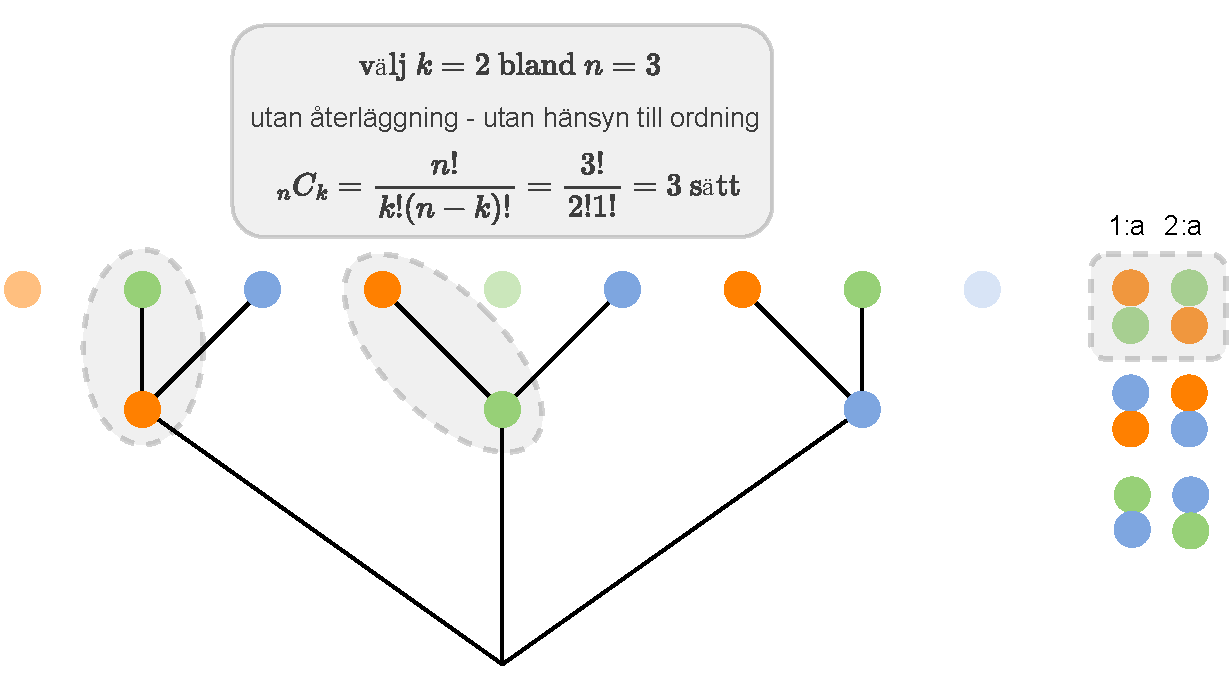
\includegraphics[scale=0.45]{figs/BallsNoReplaceWithoutOrdering}
\par\end{center}

\end{frame}

\begin{frame}{\textbf{\textcolor{orange}{Credits}}}

Dessa slides skapades för kursen statistik och dataanalys 1 av Mattias
Villani HT 2023, och har modifierats av Oscar Oelrich för statistik
och dataanalys 1 VT 2024.

\end{frame}

\end{document}
